% this is a beamer presentation file

\documentclass{beamer}
\usepackage{graphicx}
\usepackage{amsmath}
\usepackage{amssymb}
\usepackage{amsthm}
\usepackage{amsfonts}
\usepackage{amscd}
\usepackage{color}
\usepackage{enumerate}
\usepackage{hyperref}
\usepackage{url}
\usepackage{verbatim}
\usepackage{listings}
\usepackage{tikz}
\usepackage{pgfplots}
\pgfplotsset{compat=1.18}
\usepackage{blindtext}

\title{PHYS 420: Ray Tracing Demonstration and Discussion}
\author{Ashtan Mistal}
\institute{University of British Columbia}
\date{\today}

\begin{document}

  \begin{frame}
    \titlepage
  \end{frame}

% Introduce the audience to what ray tracing is

  \begin{frame}
    \frametitle{What is Ray Tracing?}
    \begin{itemize}
      \item Ray Tracing is a method used to model the propagation of light through a scene more accurately than traditional techniques
      \item Familiar applications of ray tracing include computer graphics (such as video games, movies, and simulations), astronomy, and optics
    \end{itemize}
  \end{frame}

  % area light sources can be used in ray tracing; they are not possible in conventional lighting models without a lot of work (usually involving a lot of point lights)
  % soft shadows (hard shadows can be calculated without ray tracing -- use A4 demo for this)
  % ambient occlusion
  % global illumination
  % reflections (without ray tracing, reflections become a more complicated problem). This is a good place to mention that ray tracing is not just for rendering, but also for physics.
  % without ray tracing, it's easy to get single reflections, but not multiple reflections.

  % there are tricks to get around some of these problems, but they are not as accurate as ray tracing
  % subsurface scattering: ray tracing is the only way to get this effect
  % subsurface scattering (scattering on the inside of an object)
  % -> in skin, gemstones, leaves on trees, etc. (basically anything that is translucent or slightly translucent)

  \begin{frame}
    \frametitle{How do traditional lighting methods work?}

    Let's briefly go over how lighting is calculated in flat shading and Phong shading.

  \end{frame}


  \begin{frame}
    \frametitle{Flat Shading}
    \begin{itemize}
      \item Flat shading is a method of shading that uses a single color for each polygon in a scene
      \item The color of each polygon is determined by the color of the light source that is closest to the polygon
      \item This method is fast, but it does not take into account the position of the viewer
    \end{itemize}
  \end{frame}

  % include the following image: https://upload.wikimedia.org/wikipedia/commons/6/6b/Phong_components_version_4.png
  \begin{frame}
    \frametitle{Phong Shading}
    \begin{itemize}
      \item Phong shading is a method of shading that uses a combination of ambient, diffuse, and specular lighting.
      \item This model interpolates the normal vector at each vertex of a polygon, and then uses the interpolated normal vector to calculate the lighting at each pixel.
    \end{itemize}
    % \write18{wget https://upload.wikimedia.org/wikipedia/commons/6/6b/Phong_components_version_4.png}

    \begin{figure}
      \centering
      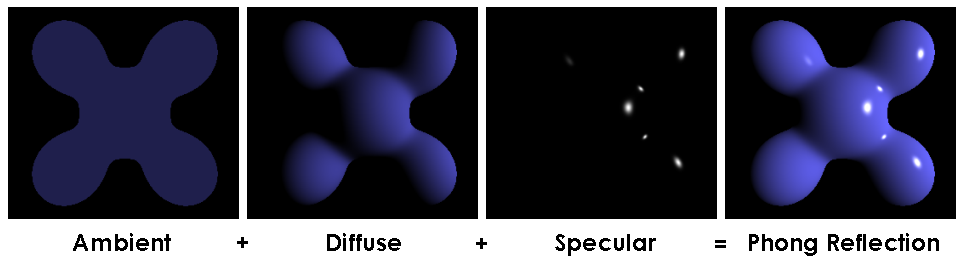
\includegraphics[width=0.8\textwidth]{Phong_components_version_4.png}
      \caption{Components of a Phong shading model. Source: Phong shading, Wikipedia}
      \label{fig:phong}
    \end{figure}

  \end{frame}

  \begin{frame}
    \frametitle{Phong Shading - Details}
    How does Phong shading use the normal vector to calculate the lighting at each pixel?

    Phong shading approximates the BRDF (bidirectional reflectance distribution function) of the surface using the ambient, diffuse, and specular lighting components.

    The details of this function are not important, but we can think of it as a function that defines exactly how light is reflected off a given surface, through the components we described above and on the previous slide.

    % \hfill

    % From Wikipedia:

    % \[ {\displaystyle f_{\text{r}}(\omega _{\text{i}},\,\omega _{\text{r}})\,=\,{\frac {\mathrm {d} L_{\text{r}}(\omega _{\text{r}})}{\mathrm {d} E_{\text{i}}(\omega _{\text{i}})}}\,=\,{\frac {1}{L_{\text{i}}(\omega _{\text{i}})\cos \theta _{\text{i}}}}{\frac {\mathrm {d} L_{\text{r}}(\omega _{\text{r}})}{\mathrm {d} \omega _{\text{i}}}}} \]

    % where where $ L $ is radiance, or power per unit solid-angle-in-the-direction-of-a-ray per unit projected-area-perpendicular-to-the-ray, $ E $ is irradiance, or power per unit surface area, and $ \theta _{\text{i}} $ is the angle between $ \omega _{\text{i}} $ and the surface normal, $ \mathbf {n} $. The index $ {\text{i}} $ indicates incident light, whereas the index $ {\text{r}} $ indicates reflected light.

  \end{frame}

  \begin{frame}
    \frametitle{Phong Shading - Details}
    \begin{itemize}
      \item The ambient component is the same for all pixels in the scene
      \item The diffuse component is calculated using the dot product of the normal vector and the vector from the light source to the pixel.
      The intensity of this component is independent of the viewer's position.

      \begin{figure}
        \centering
        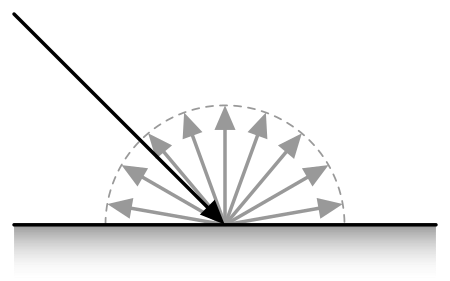
\includegraphics[width=0.7\textwidth]{diffuse.png}
        % https://upload.wikimedia.org/wikipedia/commons/thumb/4/4e/BRDF_diffuse.svg/450px-BRDF_diffuse.svg.png
        \caption{Diffuse component. Source: Bidirectional reflectance distribution function, Wikipedia}\label{fig:diffuse}
      \end{figure}
    \end{itemize}

  \end{frame}

  \begin{frame}{Phong Shading - Details}

    \begin{itemize}
      \item The specular component is calculated using the dot product of the normal vector and the vector from the viewer to the pixel.
      This can be thought of as the \("\)shininess\("\) of the surface.

      \begin{figure}
        \centering
        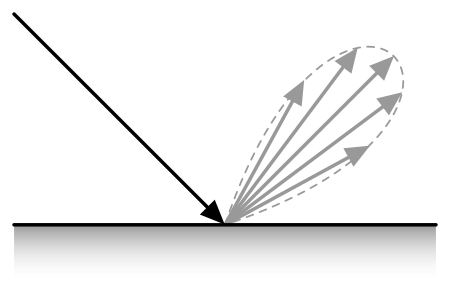
\includegraphics[width=0.7\textwidth]{specular.png}
        % https://upload.wikimedia.org/wikipedia/commons/thumb/f/fa/BRDF_glossy.svg/450px-BRDF_glossy.svg.png
        \caption{Specular component. Source: Bidirectional reflectance distribution function, Wikipedia}\label{fig:specular}
      \end{figure}


    \end{itemize}




  \end{frame}

  \begin{frame}
    \frametitle{What's missing from these models?}

    By using flat shading, it's pretty clear that we're missing a lot of key components.
    But, even with Phong shading, we're ignoring some crucial phenomena that occur in real life:

    \begin{itemize}
      \item Shadows (these can be approximated in addition to Phong shading, but soft shadows are not possible without ray tracing)
      \item Reflections: Here, we've seen single reflections, but not multiple reflections.
      We don't see the reflected rays bouncing off of another surface after reflecting off of one. So - No mirrors natively.
      \item Refractions: We don't see the light rays refracting when they pass through a transparent object.
      The object is either ignored by the light or treated as a solid object.
    \end{itemize}

  \end{frame}

  \begin{frame}{What's missing from these models?}

    \begin{itemize}
      \item Global illumination: We don't see the light rays bouncing off of other objects in the scene.
      We're only taking into account direct lighting and not lighting coming from other objects.
      \item Subsurface scattering: We don't see the light rays scattering on the inside of an object.
      \item Ambient occlusion: We don't see ambient light being blocked by other objects in the scene, for we set the ambient component to be the same for all pixels.
    \end{itemize}

  \end{frame}

  \begin{frame}
    \frametitle{Solving these problems without ray tracing}

    Of course, we don't have to use ray tracing to solve these problems.
    To an extent, we can use other methods to approximate these phenomena.
    For example, we can use shadow maps to approximate shadows.

    \hfill

    We won't go into the details of the methods used to solve these problems, but you can read more about them in the references at the end of this presentation if you're interested.

    \hfill

    But these methods are not perfect -- they're approximations of the real phenomena.

    \hfill

    Which brings us to ray tracing.

  \end{frame}

  \begin{frame}
    \frametitle{Ray Tracing Basics}
    \begin{itemize}
      \item Ray tracing is a method of rendering that uses rays to calculate the color of each pixel in the scene.
      \item A ray is a line that starts at a point - this could be from a light source or from another object - and extends infinitely in a particular direction through the scene.
      \item Once a ray hits an object, it is reflected or refracted depending on the material properties of the object.
      This allows us to directly determine where the light ray should go next - whether it be reflected away from the object, refracted through the object, or absorbed by the object.
      \item This process is repeated until the ray either leaves the scene, is absorbed by an object, or hits the camera.
    \end{itemize}

  \end{frame}

  \begin{frame}{Ray Tracing Basics}

    There are two kinds of ray tracing: light-based ray tracing and eye-based ray tracing.

    \hfill

    We'll be focusing on light-based ray tracing in this presentation as it makes more sense from a Physics perspective.
    In short, eye-based draws the scene from the perspective of the viewer, whereas light-based draws the scene from the perspective of the light source.
    Eye-based ray tracing is used to render 3D scenes in video games as we ignore the rays that don't reach the viewer, which is more efficient.
    Light-based ray tracing is used to render 3D scenes in movies.

  \end{frame}

  \begin{frame}
    \frametitle{The Physics of Light}
    Let's briefly go over the physics of light before we get into the details of ray tracing.
  \end{frame}

  \begin{frame}
    \frametitle{Reflection}
    \begin{itemize}
      \item Reflection is the bouncing of light off of a surface.
      \item The angle of reflection is equal to the angle of incidence.
      This is known as the law of reflection.
      \item The angle of incidence is equal to the angle between the incident ray and the normal vector of the surface. (the normal vector is a vector perpendicular to the surface)
    \end{itemize}

    % can draw a diagram on the board
  \end{frame}

  \begin{frame}{Refraction}
    \begin{itemize}
      \item Refraction is the bending of light as it passes through a medium.
      \item The light is bent according the refraction index of the medium it is transmitting from and the refraction index of the medium it is transmitting to, based on Snell's law:
      \[ n_i \sin i = n_r \sin r \]

      where \(n_i\) is the refraction index of the medium the light is transmitting from, \(n_r\) is the refraction index of the medium the light is transmitting to, \(i\) is the angle of incidence, and \(r\) is the angle of refraction.
    \end{itemize}

    % can also draw a diagram on the board for this
  \end{frame}

  \begin{frame}{Total Internal Reflection}

    If we have light that is transmitted from a medium with a higher refraction index than the light on the other side of the system, once the light is at a small enough angle, the ray will undergo total internal reflection.
    This is important for keeping in mind how light bounces around inside objects, which is how subsurface scattering occurs.

    % TODO include an image of total internal reflection

  \end{frame}

  \begin{frame}{The Physics of Light}

    Beyond the basic principles that we just covered, there are certainly more.
    But they aren't super important for us to be able to gain an understanding into what ray tracing does.

    \hfill

    As such, let's see this in practice.

  \end{frame}


  \begin{frame}{Ray Tracing}

    From this, let's go over how we can visualize the process that ray tracing occurs.
    We'll start with a basic scene, with no lights on just yet.
    This scene has enough objects that the light should be able to bounce off and around different objects in the scene.
    And, if we look closely, we'll see that many of the blocks have different textures in them.

    \hfill

    As such, light will bounce off each object differently, sending light through the scene either through diffuse reflection or specular.
    After it bounces, we see that it will reach another object, and continue to bounce off of that.

    \hfill

    What we're doing right now is tracing the path of the ray as it goes from the source, all the way until it reaches the viewer.

  \end{frame}

  \begin{frame}{How this will be demonstrated}
    Similarly to what was discussed during the 5-minute presentation, this will be demonstrated through a setup that involves a light source, in this case a projector.
    The projector will have a singular pixel (or a small group of pixels, depending on the resolution of the projector) lit up.
    This will therefore show a singular laser beam travelling throughout the scene and lighting things up as we go.

    Next, we will move on to slowly adding more lasers at random placements to slowly build up the lit scene.
  \end{frame}

  \begin{frame}{How else will this be demonstrated outside the hands-on laser demo?}

    \begin{itemize}
      \item Recreation of the hands-on demo in WebGL, available on the website
      \begin{itemize}
        \item This will be the same scene but lit up with different lighting models, from flat lighting, Gouraud shading, Phong shading, and ray traced.
        \item The ray traced demonstration will likely need to be pre-computed - It should be interactive, but not live.
        Too computationally expensive to do it live, especially with inherent machine differences.
      \end{itemize}
      \item Other pictures of comparisons and examples of various lighting models will be given - the example shown above is great for Phong shading but there's a lot to cover outside of what we can here
      \item Cool pictures!
      spheres are boring.
      Kids want to see really cool graphics in neat situations (movies, games, etc.)
    \end{itemize}

  \end{frame}

  \begin{frame}{How will we build the demonstration?}
    \begin{itemize}
      \item Projector will be sourced from IKB or supplied by myself (might buy one from Amazon and then return it if that's feasible)
      \item Source of fog for the demonstration:
      \begin{itemize}
        \item Dry ice or liquid nitrogen is not ideal as the temperature will change the reflective properties of some materials (e.g. a mirror)
        \item Some chemical reaction that produces a safe but visible cloudy gas
        \item What chemical produces the cloud in vapes?
        \item fog machine (most ideal but also most expensive)
      \end{itemize}
      \item Base of the demo will be wood with overlayed felt (the latter sourced from Michaels if unavailable here)
      \item will continue to look for wooden blocks here if they're available else Amazon will do
      \item Blocks will be coated in various materials - the exact materials are still TBD but I am playing with a few ideas
    \end{itemize}

  \end{frame}

  \begin{frame}{Applications of Ray Tracing}
    \begin{itemize}
      \item Real-time Rendering
      \begin{itemize}
        \item Video Games
        \item VR/AR
        \item Augmented Reality (AR)
      \end{itemize}
      \item Photorealistic Rendering
      \begin{itemize}
        \item Movies
        \item TV
        \item Video
        \item Advertising
      \end{itemize}
      \item Scientific Visualization
      \begin{itemize}
        \item Medical Imaging
        \item Astronomy
        \item Engineering
      \end{itemize}
    \end{itemize}

  \end{frame}

  \begin{frame}{Applications of Ray Tracing}
    \begin{itemize}
      \item Real-time Rendering
      \begin{itemize}
        \item Video Games
        \item Virtual and Augmented Reality
      \end{itemize}
      \item Photorealistic Rendering
      \begin{itemize}
        \item Movies; TV; Video; Advertising
      \end{itemize}
      \item Scientific Visualization
      \begin{itemize}
        \item Medical Imaging
        \item Astronomy
        \item Engineering
      \end{itemize}
    \end{itemize}

  \end{frame}

  \begin{frame}{Ray Tracing in Video Games}
    \begin{itemize}
      \item Ray Tracing is used in many games.
      Here's an example:
      \begin{figure}
        \centering
        \includegraphics[width=0.8\textwidth]{images/raytracing_in_video_games.png}
        \caption{Ray Tracing in Video Games}
      \end{figure}
%      \begin{itemize}
%        \item Crysis 2
%        \item Crysis 3
%        \item Battlefield 4
%        \item The Witcher 3
%        \item Star Wars Battlefront
%        \item Dishonored 2
%        \item Hitman
%        \item Deus Ex: Mankind Divided
%        \item Prey
%        \item Battlefield 1
%        \item Wolfenstein 2: The New Colossus
%        \item Metro Exodus
%        \item Far Cry 5
%        \item Assassin's Creed: Origins
%        \item The Evil Within 2
%        \item God of War
%        \item Horizon Zero Dawn
%        \item Red Dead Redemption 2
%        \item Shadow of the Tomb Raider
%        \item Battlefield V
      \end{itemize}
    \end{frame}

  \begin{frame}{Questions}
    Any questions?
  \end{frame}



\end{document}
